% !TeX program = lualatex
% Lualatex is important to render Fira fonts; with pdflatex it's just the regular one
\documentclass[12pt]{beamer}

\usetheme{metropolis}
\usepackage{appendixnumberbeamer}

% adjust the background to be completely white
\setbeamercolor{background canvas}{bg=white}

\usepackage{booktabs}
\usepackage[scale=2]{ccicons}

\usepackage{pgfplots}
\usepgfplotslibrary{dateplot}

% typeset mathematics on serif
\usefonttheme[onlymath]{serif}

% better bibliography using biber as backend
\usepackage[natbib=true,backend=biber,style=authoryear-icomp,maxbibnames=30,maxcitenames=3,uniquelist=false,giveninits=true,doi=false,url=true,dashed=false,isbn=false]{biblatex}
% shared bibliogrphy
\addbibresource{../dl4nlp-bibliography.bib}
% disable "ibid" for repeated citations
\boolfalse{citetracker}

% TODOs
\usepackage{todonotes}
\let\todox\todo
\renewcommand\todo[1]{\todox[inline]{#1}}

\definecolor{76abdf}{RGB}{118, 171, 223}

\setbeamercolor{frametitle}{bg=76abdf, fg=white}

\usepackage{xspace}
\newcommand{\themename}{\textbf{\textsc{metropolis}}\xspace}

% POS tags
\newcommand*\POS[1]{\textsubscript{\texttt{#1}}} % tag with part of speech

% parse tree
\usepackage{qtree}

% NNEts
\usepackage{tikz}
\usetikzlibrary{matrix, positioning, calc}

\tikzset{
	neuron/.style={
		draw,
		circle,
		inner sep=0pt,
		minimum width=0.75cm
	},
	layer/.style={
		matrix of nodes,
		nodes={neuron},
		row sep={between origins, 1.2cm}, %1.5cm in general, 2.5cm for backprop task
		nodes in empty cells
	}
}

% for derivatives, https://tex.stackexchange.com/a/412442
\usepackage{physics}

% code listing
\usepackage{listings}

% XML formatting; taken from https://gist.github.com/sebald/3130827
\definecolor{dkgreen}{rgb}{0,0.6,0}
\definecolor{gray}{rgb}{0.5,0.5,0.5}
\definecolor{mauve}{rgb}{0.58,0,0.82}
\definecolor{gray}{rgb}{0.4,0.4,0.4}
\definecolor{darkblue}{rgb}{0.0,0.0,0.6}
\definecolor{lightblue}{rgb}{0.0,0.0,0.9}
\definecolor{cyan}{rgb}{0.0,0.6,0.6}
\definecolor{darkred}{rgb}{0.6,0.0,0.0}
\lstset{
	basicstyle=\ttfamily\scriptsize,
	columns=fullflexible,
	showstringspaces=false,
	numbers=left,                   % where to put the line-numbers
	numberstyle=\tiny\color{gray},  % the style that is used for the line-numbers
	stepnumber=1,
	numbersep=5pt,                  % how far the line-numbers are from the code
	backgroundcolor=\color{white},      % choose the background color. You must add \usepackage{color}
	showspaces=false,               % show spaces adding particular underscores
	showstringspaces=false,         % underline spaces within strings
	showtabs=false,                 % show tabs within strings adding particular underscores
	frame=none,                   % adds a frame around the code
	rulecolor=\color{black},        % if not set, the frame-color may be changed on line-breaks within not-black text (e.g. commens (green here))
	tabsize=2,                      % sets default tabsize to 2 spaces
	captionpos=b,                   % sets the caption-position to bottom
	breaklines=true,                % sets automatic line breaking
	breakatwhitespace=false,        % sets if automatic breaks should only happen at whitespace
	title=\lstname,                   % show the filename of files included with \lstinputlisting;
	% also try caption instead of title  
	commentstyle=\color{gray}\upshape
}
\lstdefinelanguage{XML}
{
	morestring=[s][\color{mauve}]{"}{"},
	morestring=[s][\color{black}]{>}{<},
	morecomment=[s]{<?}{?>},
	morecomment=[s][\color{dkgreen}]{<!--}{-->},
	stringstyle=\color{black},
	identifierstyle=\color{lightblue},
	keywordstyle=\color{red},
	morekeywords={xmlns,xsi,noNamespaceSchemaLocation,type,id,x,y,source,target,version,tool,transRef,roleRef,objective,eventually}% list your attributes here
}


% tables with color
\usepackage{colortbl}

% from Mohsen
% the bm package
\usepackage{bm}

\definecolor{myblue}{RGB}{1,70,153}


\title{Deep Learning for Natural Language Processing}
\subtitle{Lecture 7 -- Recurrent Neural Networks}
\date{May 31, 2022}
\author{Dr.\ Ivan Habernal}
\institute{Trustworthy Human Language Technologies  \hfill 
\includegraphics[height=.8cm]{img/logo-trusthlt.pdf} \\
Department of Computer Science\\
Technical University of Darmstadt \hfill \texttt{www.trusthlt.org}}
%\titlegraphic{\hfill }

\begin{document}

\maketitle



\begin{frame}{This lecture}
	\vspace*{1cm}
	\begin{itemize}
		\item RNNs
		\item Vanishing and explosion
		\item GRUs
		\item LSTMs
		\item Application of RNNs in NLP
	\end{itemize}
\end{frame}
%%%%%%%%%%%%%%%%%%%%%%%%%%%%%%%%


\begin{frame}{Recall: MultiLayer Perceptron (MLP)}
	\centering
	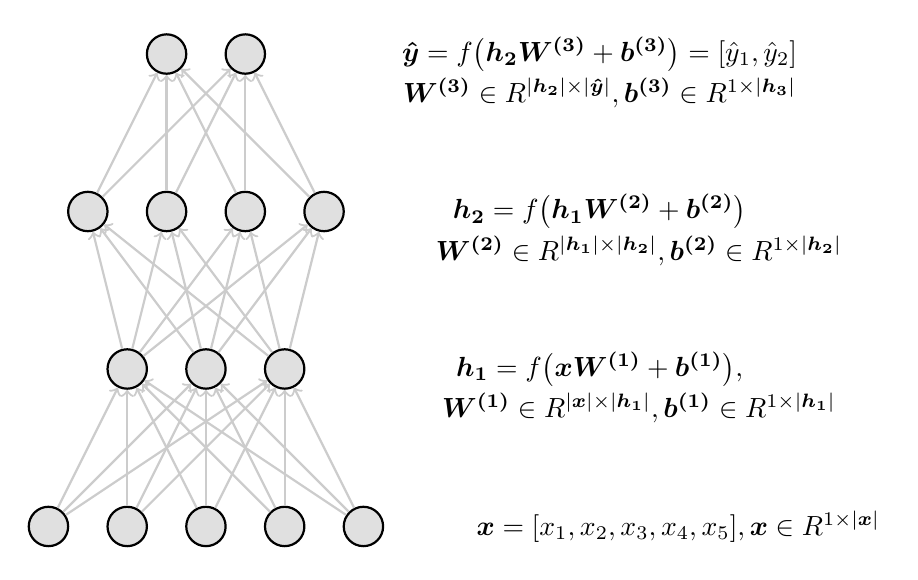
\begin{tikzpicture}
	\tikzset{node/.style={draw,circle, minimum width=0.5cm, fill=gray!20, thick}}
	\tikzset{edge/.style={draw, thick, black!20, ->}}
	
	\node(x1) at (0, 0) [node] {};
	\node(x2) at (1, 0) [node] {};
	\node(x3) at (2, 0) [node] {};
	\node(x4) at (3, 0) [node] {};
	\node(x5) at (4, 0) [node] {};
	
	\node(x_label) at (8,0.0) {$\bm{x} = [x_1, x_2, x_3, x_4, x_5], \bm{x} \in \mathbb{R}^{1 \times |\bm{x}|}$};
	
	\node(h11) at (1, 2) [node] {};
	\node(h12) at (2, 2) [node] {};
	\node(h13) at (3, 2) [node] {};
	
	\node(h1_label) at (7,2) {$\bm{h_1}= f \big( \bm{x}\bm{W^{(1)}} + \bm{b^{(1)}} \big), $};
	\node(h1_dim) at (7.5,1.5) {$\bm{W^{(1)}} \in \mathbb{R}^{|\bm{x}| \times |\bm{h_1}|}, \bm{b^{(1)}} \in \mathbb{R}^{1 \times |\bm{h_1}|}  $};
	
	\node(h21) at (0.5, 4) [node] {};
	\node(h22) at (1.5, 4) [node] {};
	\node(h23) at (2.5, 4) [node] {};
	\node(h24) at (3.5, 4) [node] {};
	
	\node(h2_label) at (7,4) {$\bm{h_2}= f \big( \bm{h_1} \bm{W^{(2)}} + \bm{b^{(2)}} \big)$};
	\node(h2_dim) at (7.5,3.5) {$ \bm{W^{(2)}} \in \mathbb{R}^{|\bm{h_1}| \times |\bm{h_2}|}, \bm{b^{(2)}} \in \mathbb{R}^{1 \times |\bm{h_2}|} $};
	
	\node(y1) at (1.5, 6) [node] {};
	\node(y2) at (2.5, 6) [node] {};
	
	
	\node(h2_label) at (7,6) {$\bm{\hat{y}}= f \big( \bm{h_2}\bm{W^{(3)}} + \bm{b^{(3)}} \big) = [\hat{y}_1, \hat{y}_2] $};
	\node(h2_dim) at (7,5.5) { $\bm{W^{(3)}} \in \mathbb{R}^{|\bm{h_2}| \times |\bm{\hat{y}}|}, \bm{b^{(3)}} \in \mathbb{R}^{1 \times |\bm{h_3}|} $};
	
	
	
	\draw[edge] (x1) -- (h11);
	\draw[edge] (x2) -- (h11);
	\draw[edge] (x3) -- (h11);
	\draw[edge] (x4) -- (h11);
	\draw[edge] (x5) -- (h11);
	
	
	\draw[edge] (x1) -- (h12);
	\draw[edge] (x2) -- (h12);
	\draw[edge] (x3) -- (h12);
	\draw[edge] (x4) -- (h12);
	\draw[edge] (x5) -- (h12);
	
	\draw[edge] (x1) -- (h13);
	\draw[edge] (x2) -- (h13);
	\draw[edge] (x3) -- (h13);
	\draw[edge] (x4) -- (h13);
	\draw[edge] (x5) -- (h13);
	
	\draw[edge] (h11) -- (h21);
	\draw[edge] (h11) -- (h22);
	\draw[edge] (h11) -- (h23);
	\draw[edge] (h11) -- (h24);
	
	
	\draw[edge] (h12) -- (h21);
	\draw[edge] (h12) -- (h22);
	\draw[edge] (h12) -- (h23);
	\draw[edge] (h12) -- (h24);
	
	\draw[edge] (h13) -- (h21);
	\draw[edge] (h13) -- (h22);
	\draw[edge] (h13) -- (h23);
	\draw[edge] (h13) -- (h24);
	
	\draw[edge] (h21) -- (y1);
	\draw[edge] (h22) -- (y1);
	\draw[edge] (h23) -- (y1);
	\draw[edge] (h24) -- (y1);
	
	\draw[edge] (h21) -- (y2);
	\draw[edge] (h22) -- (y2);
	\draw[edge] (h23) -- (y2);
	\draw[edge] (h24) -- (y2);
	
	
	\end{tikzpicture}
	
	
\end{frame}
\begin{frame}{Recall: Feedforward}
	\centering
	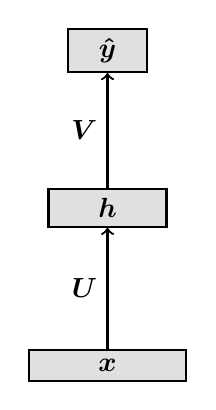
\begin{tikzpicture}
	\tikzset{layer/.style={draw,rectangle, fill=gray!20, thick}}
	\tikzset{edge/.style={->, thick}}
	
	\node(x) at (0,0) [layer, minimum width=2cm] {$\bm{x}$};
	\node(h) at (0,2) [layer, minimum width=1.5cm] {$\bm{h}$};
	\node(y_hat) at (0,4) [layer, minimum width=1cm] {$\bm{\hat{y}}$};
	
	
	\draw[edge](x) --node[left]{$\bm{U}$} (h);
	\draw[edge](h) -- node[left]{$\bm{V}$} (y_hat);
	
	
	\end{tikzpicture}
	
	
\end{frame}
\begin{frame}{Motivation}

Text is a \textbf{sequence} of symbols

Symbols = characters, words, etc.

\begin{example}
input = ``a persian cat on the mat'' $\longrightarrow$ \\ input = $\big( x_1=$a, $x_2=$persian, $x_3=$cat, $x_4=$sat, $x_5=$on, $x_6=$the, $x_7=$mat$ \big) $ 
\end{example}

\bigskip

Symbols are related to each other in text, so should symbols' representations

\end{frame}
\begin{frame}{Recurrent}
	\centering
	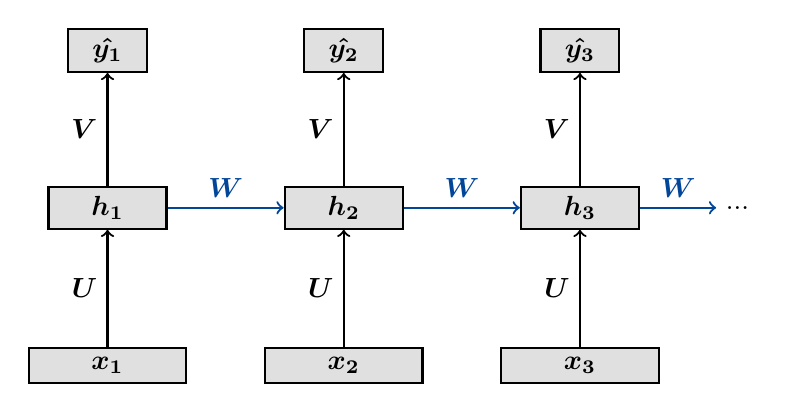
\begin{tikzpicture}
	\tikzset{layer/.style={draw,rectangle, fill=gray!20, thick}}
	\tikzset{edge/.style={->, thick}}
	
	\node(x1) at (0,0) [layer, minimum width=2cm] {$\bm{x_1}$};
	\node(h1) at (0,2) [layer, minimum width=1.5cm] {$\bm{h_1}$};
	\node(y1_hat) at (0,4) [layer, minimum width=1cm] {$\bm{\hat{y_1}}$};
	\draw[edge](x1) -- node[left]{$\bm{U}$} (h1);
	\draw[edge](h1) -- node[left]{$\bm{V}$} (y1_hat);
	
	
	\node(x2) at (3,0) [layer, minimum width=2cm] {$\bm{x_2}$};
	\node(h2) at (3,2) [layer, minimum width=1.5cm] {$\bm{h_2}$};
	\node(y2_hat) at (3,4) [layer, minimum width=1cm] {$\bm{\hat{y_2}}$};
	\draw[edge](x2) -- node[left]{$\bm{U}$} (h2);
	\draw[edge](h2) -- node[left]{$\bm{V}$} (y2_hat);
	
	\node(x3) at (6,0) [layer, minimum width=2cm] {$\bm{x_3}$};
	\node(h3) at (6,2) [layer, minimum width=1.5cm] {$\bm{h_3}$};
	\node(y3_hat) at (6,4) [layer, minimum width=1cm] {$\bm{\hat{y_3}}$};
	\draw[edge](x3) -- node[left]{$\bm{U}$} (h3);
	\draw[edge](h3) -- node[left]{$\bm{V}$} (y3_hat);
	
	\node(etc) at (8,2) [] {...};
	
	\draw[edge, myblue] (h1) -- node[above]{$\bm{W}$} (h2);
	\draw[edge,myblue] (h2) -- node[above]{$\bm{W}$} (h3);
	\draw[edge,myblue] (h3) -- node[above]{$\bm{W}$} (etc);
	
	\end{tikzpicture}
\end{frame}
\begin{frame}{Recurrent}
	\centering
	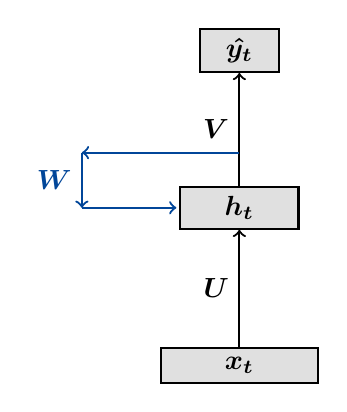
\begin{tikzpicture}
	\tikzset{layer/.style={draw,rectangle, fill=gray!20, thick}}
	\tikzset{edge/.style={->, thick}}
	
	
	\node(xt) at (0,0) [layer, minimum width=2cm] {$\bm{x_t}$};
	\node(ht) at (0,2) [layer, minimum width=1.5cm] {$\bm{h_t}$};
	\node(yt_hat) at (0,4) [layer, minimum width=1cm] {$\bm{\hat{y_t}}$};
	\draw[edge](xt) -- node[left]{$\bm{U}$} (ht);
	\draw[edge](ht) -- node[left]{$\bm{V}$} (yt_hat);
	
	\draw[edge, myblue] (0,2.7) -- (-2,2.7);
	\draw[edge, myblue] (-2,2.7) -- node[left]{$\bm{W}$} (-2,2);
	\draw[edge, myblue] (-2,2) --  (-0.8,2); 
%	\draw[edge, myblue] (-0.2,1.3) --  (-0.2,1.7);
	\end{tikzpicture}
\end{frame}
\begin{frame}{Recurrent}

Input = a sequence of vectors = $[\bm{x_1},\bm{x_2},\bm{x_3},...,\bm{x_n}]$, $\bm{x_t} \in \mathbb{R}^{1\times |x|}$
\begin{equation*}
\bm{h_t} =  f \big( \bm{x_t}U + \textcolor{myblue}{\bm{h_{t-1}}W} + \bm{b_h}  \big)
\end{equation*}
$|h|$ is the dimensionality of hidden states

$$\bm{U} \in \mathbb{R}^{|x|\times |h|}
\qquad
\bm{W} \in \mathbb{R}^{|h|\times |h|}
\qquad
\bm{b_h} \in \mathbb{R}^{1\times |h|}
$$

\begin{equation*}
\bm{\hat{y}_t} =  g \big( \bm{h_t}V + \bm{b_{\hat{y}}}  \big)
\end{equation*}

$$
\bm{V} \in \mathbb{R}^{|h|\times |\hat{y}|}
\qquad \bm{b_{\hat{y}}} \in \mathbb{R}^{1\times |\hat{y}|}
$$

\end{frame}

\begin{frame}{Training}
Input = $[\bm{x_1},..., \bm{x_n}]$, $\longrightarrow$ output = $[\bm{y_1},..., \bm{y_n}]$


The loss of sequence prediction is the mean of step losses
\begin{equation*}
\ell = \frac{1}{n} \sum_{t=1}^n \ell_t(\bm{y_t}, \bm{\hat{y}_t})
\end{equation*}

\bigskip

Backpropagation to compute gradients

SGD to update parameters

\end{frame}
\begin{frame}{Some Properties of RNNs}
Hidden state is known also as memory

In principle, the hidden state represents information from the first step until the current step conditioned on current input symbol

So RNNs can capture left-to-right order of input symbols

\end{frame}

\begin{frame}{Example}
	\begin{itemize}
		\item input = $\big( x1=$a, $x2=$persian, $x3=$cat$ \big) $ $\longrightarrow$ \\ output = $ \big( y_1=$DET, $y_2=$ADJ, $y_3=$NOUN \big) 
		\item Assume following embeddings for input:
		\begin{itemize}
			\item $\bm{x_1} = \begin{bmatrix} 1 & 0 & 0 \end{bmatrix}$
			\item $\bm{x_2} = \begin{bmatrix} 1 & 1 & 2 \end{bmatrix}$
			\item $\bm{x_3} = \begin{bmatrix}  1 & -1 & 1 \end{bmatrix}$
		\end{itemize}
		\item Assume following 1-hot vectors for output:
		\begin{itemize}
			\item $\bm{y_1} = \begin{bmatrix} 1 & 0 & 0 & 0\end{bmatrix}$
			\item $\bm{y_2} = \begin{bmatrix} 0 & 1 & 0 & 0\end{bmatrix}$
			\item $\bm{y_3} = \begin{bmatrix} 0 & 0 & 0 & 1\end{bmatrix}$
		\end{itemize}
	\end{itemize}
\end{frame}

\begin{frame}{Example}
	\begin{itemize}
		\item The sequence prediction task can be solved by RNNs
		\item Let $|h| = 2$, $f$ be \texttt{ReLU}, and $g$ be \texttt{softmax}
		\item We initialize the RNN's parameters by random values
		\begin{itemize}
			\item $\bm{U} = \begin{bmatrix}  1 & 1 \\ 2 & 0 \\ 0.5 & 1 \end{bmatrix}$
			\item $\bm{W} = \begin{bmatrix}  0 & 1 \\ 1 & 0 \end{bmatrix}$
			\item $\bm{V} = \begin{bmatrix}  0 & 1 & 0 & 0  \\ 1 & 0 & \frac{1}{3} & 1 \end{bmatrix}$
			\item $\bm{b_h},\bm{b_{\hat{y}}}$ zero vectors
			\item $\bm{h_0} = \begin{bmatrix} 0 & 0 \end{bmatrix}$
		\end{itemize}
	\end{itemize}
\end{frame}

\begin{frame}
	\centering
	\small
	\scalebox{0.7}{
		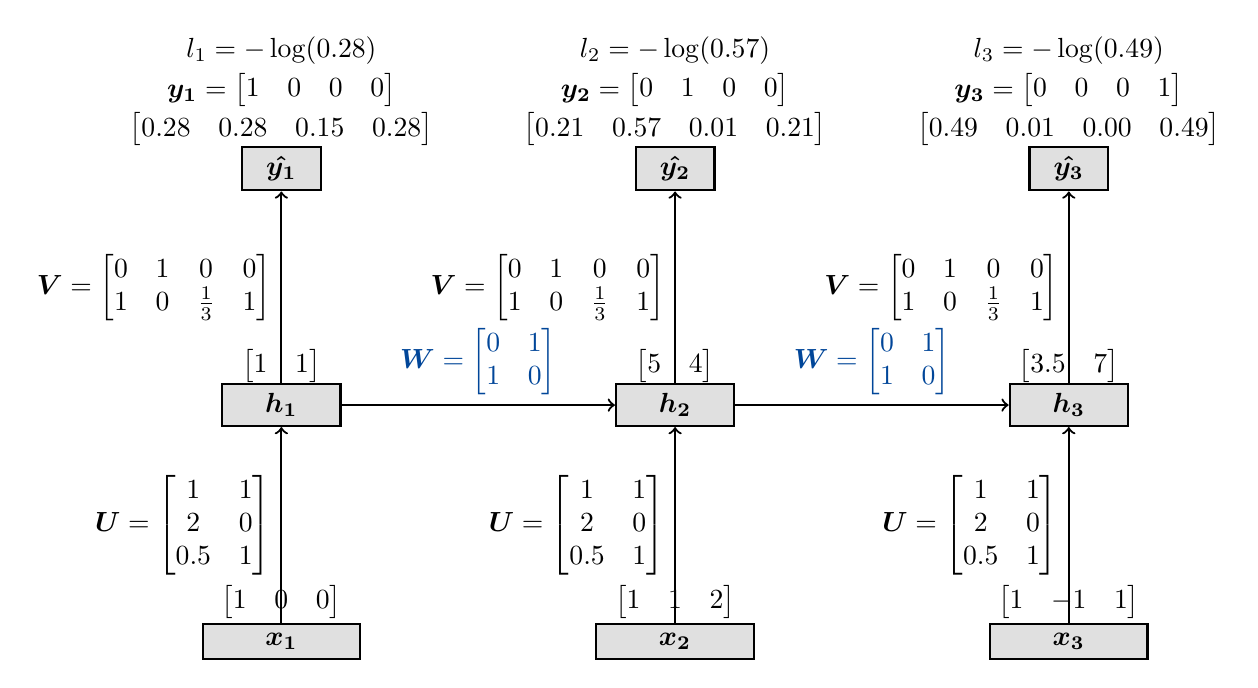
\begin{tikzpicture}
		\tikzset{layer/.style={draw,rectangle, fill=gray!20, thick}}
		\tikzset{edge/.style={->, thick}}
		
		\node(x1) at (0,0) [layer, minimum width=2cm] {$\bm{x_1}$};
		\node(x1_value) at (0,0.5) {$\begin{bmatrix} 1 & 0 & 0 \end{bmatrix}$};
		\node(h1) at (0,3) [layer, minimum width=1.5cm] {$\bm{h_1}$};
		\node(h1_value) at (0,3.5) {$\begin{bmatrix}1 & 1\end{bmatrix}$};
		\node(y1_hat) at (0,6) [layer, minimum width=1cm] {$\bm{\hat{y_1}}$};
		\node(y_hat_value) at (0,6.5) {$\begin{bmatrix}0.28 & 0.28 & 0.15 & 0.28\end{bmatrix}$};
		\draw[edge](x1) -- node[left]{$\bm{U} = \begin{bmatrix}  1 & 1 \\ 2 & 0 \\ 0.5 & 1 \end{bmatrix}$} (h1);
		\draw[edge](h1) -- node[left]{$\bm{V} = \begin{bmatrix}  0 & 1 & 0 & 0  \\ 1 & 0 & \frac{1}{3} & 1 \end{bmatrix} $} (y1_hat);
		
		
		\node(x2) at (5,0) [layer, minimum width=2cm] {$\bm{x_2}$};
		\node(x2_value) at (5,0.5) {$ \begin{bmatrix}1 & 1 & 2\end{bmatrix}$};
		\node(h2) at (5,3) [layer, minimum width=1.5cm] {$\bm{h_2}$};
		\node(h2_value) at (5,3.5) {$ \begin{bmatrix}5 & 4\end{bmatrix}$};
		\node(y2_hat) at (5,6) [layer, minimum width=1cm] {$\bm{\hat{y_2}}$};
		\node(y2_hat_value) at (5,6.5) {$ \begin{bmatrix}0.21 & 0.57 & 0.01 & 0.21 \end{bmatrix}$}; 
		

		\draw[edge](x2) -- node[left]{$\bm{U} = \begin{bmatrix}  1 & 1 \\ 2 & 0 \\ 0.5 & 1 \end{bmatrix}$} (h2);
		\draw[edge](h2) -- node[left]{$\bm{V} = \begin{bmatrix}  0 & 1 & 0 & 0  \\ 1 & 0 & \frac{1}{3} & 1 \end{bmatrix} $} (y2_hat);
		\draw[edge](h1) -- node[above]{\textcolor{myblue}{$\bm{W} =  \begin{bmatrix}  0 & 1 \\ 1 & 0 \end{bmatrix} $}} (h2);
		
		
		\node(x3) at (10,0) [layer, minimum width=2cm] {$\bm{x_3}$};
		\node(x3_value) at (10,0.5) {$ \begin{bmatrix}1 & -1 & 1 \end{bmatrix}$};
		\node(h3) at (10,3) [layer, minimum width=1.5cm] {$\bm{h_3}$};
		\node(h3_value) at (10,3.5) {$ \begin{bmatrix} 3.5 & 7 \end{bmatrix}$};
		\node(y3_hat) at (10,6) [layer, minimum width=1cm] {$\bm{\hat{y_3}}$};
		\node(y3_hat_value) at (10,6.5) {$ \begin{bmatrix}0.49 & 0.01 & 0.00 & 0.49 \end{bmatrix}$};
		% 7  3.5  7/3  7 -> 0.49 0.01 0.00 0.49
		\draw[edge](x3) -- node[left]{$\bm{U} = \begin{bmatrix}  1 & 1 \\ 2 & 0 \\ 0.5 & 1 \end{bmatrix}$} (h3);
		\draw[edge](h3) -- node[left]{$\bm{V} = \begin{bmatrix}  0 & 1 & 0 & 0  \\ 1 & 0 & \frac{1}{3} & 1 \end{bmatrix} $} (y3_hat);
		\draw[edge](h2) -- node[above]{\textcolor{myblue}{$\bm{W} =  \begin{bmatrix}  0 & 1 \\ 1 & 0 \end{bmatrix} $}} (h3);
		
		\node(y1_value) at (0,7) {
			$ \bm{y_1} = \begin{bmatrix} 1 &  0 & 0 & 0 \end{bmatrix}$}; 
		\node(y2_value) at (5,7) {
			$ \bm{y_2} = \begin{bmatrix} 0 &  1 & 0 & 0 \end{bmatrix}$}; 
		\node(y3_value) at (10,7) {
			$ \bm{y_3} =  \begin{bmatrix} 0 &  0 & 0 & 1 \end{bmatrix}$}; 
		
		\node(l1) at (0,7.5) {
			$ l_1 = - \log (0.28 )$}; 
		
		\node(l2) at (5,7.5) {
			$ l_2 = - \log (0.57 )$}; 
		
		\node(l3) at (10,7.5) {
			$ l_3 = - \log (0.49 )$}; 
		
		\end{tikzpicture}
}
\begin{align*}
\bm{h_t} = \mathrm{ReLU} \big( \bm{x_tU} + \bm{h_{t-1}W}+\bm{b_h} \big)
\qquad
\bm{\hat{y}_t} = \mathrm{softmax} \big( \bm{h_t}\bm{V} + \bm{b_{\hat{y}}} \big)
\\
\ell = - \frac{1}{3} (\log (0.28) + \log(0.57) + \log(0.49)
\end{align*}

%\node(y_hat_formula) at (5,-2.5) {$\bm{\hat{y}_t} = \texttt{softmax} \big( \bm{h_t}\bm{V} + \bm{b_{\hat{y}}} \big) $};
%\node(l) at (5,-3) {
%	$ \ell = \frac{-1}{3} (\log (0.28) + \log(0.57) + \log(0.49) $}; 



\end{frame}



\begin{frame}{Updating Parameters}
	\begin{itemize}
		\item Computation of gradients is similar as standard MLP.
		\item Keep in mind the parameters of RNNs are shared through time steps. 
		\item Sometime backprop for RNNs is called backprop through time (BPTT). 
		\item No need to go through its details as DL frameworks compute gradients. 
		\item If you would like to compute gradients brute-force, you can do that numerically. 
		\begin{itemize}
			\item for each weight $w$, compute $\frac{\text{Loss}(w+h) - \text{Loss}(w)}{h}$, 
			\item weight update after gradient computation is as in SGD $w \longleftarrow w - \alpha \frac{\partial \text{Loss}}{\partial w}$
		\end{itemize}
	\end{itemize}
\end{frame}

\begin{frame}{Updating Parameters}
	\begin{itemize}
		\item RNNs can be seen as a very very deep neural model with sparse and skip connections
		\item The output of last steps are calculated based on the hidden state vectors at early steps
		\item Recall 1:
		\begin{equation*}
		\begin{split}
		\bm{z^{(h)}_t} & = \bm{x_t}U + \bm{h_{t-1}}W + \bm{b_h} \\
		\bm{h_t} & =  f \big( \bm{z^{(h)}_t} \big) \\
		\end{split}
		\end{equation*}
		\item Recall 2:
		\begin{equation*}
		\begin{split}
		\bm{z^{(\hat{y})}_t} & = \bm{h_t}V + \bm{b_{\hat{y}}}  \\ 
		\bm{\hat{y}_t} & =  g \big(  \bm{z^{(\hat{y})}_t} \big) 
		\end{split}
		\end{equation*}
		
	\end{itemize}    
\end{frame}

\begin{frame}{Updating Parameters}
	\centering
	\begin{itemize}
		\item Recall 1:
		\begin{equation*} \bm{z^{(h)}_t}  = \bm{x_t}U + \bm{h_{t-1}}W + \bm{b_h}
		\end{equation*}
		\begin{equation*}
		\bm{h_t}  =  f\big( \bm{z^{(h)}_t} \big)
		\end{equation*}
		\item Recall 2:
		\begin{equation*}
		\bm{z^{(\hat{y})}_t} = \bm{h_t}V + \bm{b_{\hat{y}}}  
		\end{equation*}
		\begin{equation*}
		\bm{\hat{y}_t}  =  g\big(  \bm{z^{(\hat{y})}_t} \big) 
		\end{equation*}
	\end{itemize}    
\end{frame}

\begin{frame}{Updating Parameters}
	\centering
	\begin{itemize}
		\item If we have only two steps: 
		\begin{equation*}
		\frac{\partial \text{Loss}}{ \partial \bm{W}} 
		= \sum_{t=1}^{2}   \frac{\partial \ell_t}{\partial \bm{W}} = \frac{\partial \ell_1}{\partial \bm{W}}  + \frac{\partial \ell_2}{\partial \bm{W}}  
		\end{equation*}
		\begin{equation*}
		\frac{\partial \ell_1}{\partial \bm{W}}  = 
		\frac{\partial \ell_1}{\partial \bm{\hat{y_1}}} \frac{\partial \bm{\hat{y_1}}}{\partial \bm{z^{(\hat{y})}_1}}  
		\frac{\partial \bm{z^{(\hat{y})}_1}}{\partial  \bm{h_1}}  
		\frac{\partial \bm{h_1}}{\partial \bm{z^{(h)}_1}}
		\frac{\partial \bm{z^{(h)}_1}}{\partial \bm{W}}  \propto   \textcolor{myblue}{\frac{\partial \bm{h_1}}{\partial \bm{z^{(h)}_1}}}
		\end{equation*}
		\begin{equation*}
		\frac{\partial \ell_2}{\partial \bm{W}}  = 
		\frac{\partial \ell_2}{\partial \bm{\hat{y_2}}} \frac{\partial \bm{\hat{y_2}}}{\partial \bm{z^{(\hat{y})}_2}}  
		\frac{\partial \bm{z^{(\hat{y})}_2}}{\partial  \bm{h_2}}  
		\frac{\partial \bm{h_2}}{\partial \bm{z^{(h)}_2}}\bm{h_1}\frac{\partial \bm{h_1}}{\partial \bm{z^{(h)}_1}}
		\frac{\partial \bm{z^{(h)}_1}}{\partial \bm{W}} \propto  
		\textcolor{myblue}{
			\frac{\partial \bm{h_2}}{\partial \bm{z^{(h)}_2}}\frac{\partial \bm{h_1}}{\partial \bm{z^{(h)}_1}}
		}
		\end{equation*}
		
	\end{itemize}    
\end{frame}


\begin{frame}{Updating Parameters}
	\centering
	\begin{itemize}
		\item If we have  three steps: 
		\begin{equation*}
		\frac{\partial \text{Loss}}{ \partial \bm{W}} 
		= \sum_{t=1}^{3}   \frac{\partial \ell_t}{\partial \bm{W}} = \frac{\partial \ell_1}{\partial \bm{W}}  + \frac{\partial \ell_2}{\partial \bm{W}} + \frac{\partial \ell_3}{\partial \bm{W}}
		\end{equation*}
		\begin{equation*}
		\frac{\partial \ell_1}{\partial \bm{W}}  \propto   \textcolor{myblue}{\frac{\partial \bm{h_1}}{\partial \bm{z^{(h)}_1}}}
		\end{equation*}
		\begin{equation*}
		\frac{\partial \ell_2}{\partial \bm{W}}  \propto  
		\textcolor{myblue}{
			\frac{\partial \bm{h_2}}{\partial \bm{z^{(h)}_2}}\frac{\partial \bm{h_1}}{\partial \bm{z^{(h)}_1}}
		}
		\end{equation*}
		\begin{equation*}
		\frac{\partial \ell_3}{\partial \bm{W}}  \propto  
		\textcolor{myblue}{
			\frac{\partial \bm{h_3}}{\partial \bm{z^{(h)}_3}}\frac{\partial \bm{h_2}}{\partial \bm{z^{(h)}_2}}\frac{\partial \bm{h_1}}{\partial \bm{z^{(h)}_1}}
		}
		\end{equation*}     
	\end{itemize}    
\end{frame}

\begin{frame}{Updating Parameters}
	\centering
	\begin{itemize}
		\item If we have  $n$ steps: 
		\begin{equation*}
		\frac{\partial \text{Loss}}{ \partial \bm{W}} 
		= \sum_{t=1}^{3}   \frac{\partial \ell_t}{\partial \bm{W}} = \frac{\partial \ell_1}{\partial \bm{W}}  + \frac{\partial \ell_2}{\partial \bm{W}} + \frac{\partial \ell_3}{\partial \bm{W}}
		\end{equation*}
		\begin{equation*}
		\frac{\partial \ell_1}{\partial \bm{W}}  \propto   \textcolor{myblue}{\frac{\partial \bm{h_1}}{\partial \bm{z^{(h)}_1}}}
		\end{equation*}
		\begin{equation*}
		\frac{\partial \ell_2}{\partial \bm{W}}  \propto  
		\textcolor{myblue}{
			\frac{\partial \bm{h_2}}{\partial \bm{z^{(h)}_2}}\frac{\partial \bm{h_1}}{\partial \bm{z^{(h)}_1}}
		}
		\end{equation*}
		\begin{equation*}
		\frac{\partial \ell_3}{\partial \bm{W}}  \propto  
		\textcolor{myblue}{
			\frac{\partial \bm{h_3}}{\partial \bm{z^{(h)}_3}}\frac{\partial \bm{h_2}}{\partial \bm{z^{(h)}_2}}\frac{\partial \bm{h_1}}{\partial \bm{z^{(h)}_1}}
		}
		\end{equation*}
		\begin{equation*}
		...
		\end{equation*}
		\begin{equation*}
		\frac{\partial \ell_n}{\partial \bm{W}}  \propto  
		\textcolor{myblue}{
			\frac{\partial \bm{h_n}}{\partial \bm{z^{(h)}_n}} ...\frac{\partial \bm{h_3}}{\partial \bm{z^{(h)}_3}}\frac{\partial \bm{h_2}}{\partial \bm{z^{(h)}_2}}\frac{\partial \bm{h_1}}{\partial \bm{z^{(h)}_1}}
		}
		\end{equation*}     
	\end{itemize}    
\end{frame}
\begin{frame}{Exploding Gradients}
	\begin{itemize}
		\item Given: 
		\begin{equation*}
		\frac{\partial \ell_n}{\partial \bm{W}}  \propto  
		\textcolor{myblue}{
			\frac{\partial \bm{h_n}}{\partial \bm{z^{(h)}_n}} ...\frac{\partial \bm{h_3}}{\partial \bm{z^{(h)}_3}}\frac{\partial \bm{h_2}}{\partial \bm{z^{(h)}_2}}\frac{\partial \bm{h_1}}{\partial \bm{z^{(h)}_1}}
		}
		\end{equation*}     
		if all the gradients in the chain are greater than one then their multiplications explodes
		\begin{equation*}
		\frac{\partial \ell_n}{\partial \bm{W}} = \text{NaN}
		\end{equation*}
	\end{itemize}
\end{frame}
\begin{frame}{Vanishing Gradients}
	\begin{itemize}
		\item Given: 
		\begin{equation*}
		\frac{\partial \ell_n}{\partial \bm{W}}  \propto  
		\textcolor{myblue}{
			\frac{\partial \bm{h_n}}{\partial \bm{z^{(h)}_n}} ...\frac{\partial \bm{h_3}}{\partial \bm{z^{(h)}_3}}\frac{\partial \bm{h_2}}{\partial \bm{z^{(h)}_2}}\frac{\partial \bm{h_1}}{\partial \bm{z^{(h)}_1}}
		}
		\end{equation*}     
		if one of the gradients in the chain is close to zero or all gradients are less than one then their multiplications vanishes
		\begin{equation*}
		\frac{\partial \ell_n}{\partial \bm{W}} = 0.0
		\end{equation*}
	\end{itemize}
\end{frame}

\begin{frame}{Vanishing and Exploding Gradients}
	\begin{itemize}
		\item Why are such gradients a problem? 
		\item  In case of exploding gradients,  the learning is very unstable
		\item The last steps become independent from the early steps 
		\item The prediction at each step is conditioned only on a few previous steps 
		\item These problems also happen in MLPs with many hidden layer where we use the Sigmoid activation function
		
	\end{itemize}
\end{frame}

\begin{frame}{Vanishing and Exploding Gradients}
	
	When model and training suffer:
	\begin{itemize}
		\item a very high loss on training set or no learning
		\item large changes in loss on each update due to the models instability
		\item loss becomes NaN during training
		\item model weights grow exponentially during training (explosion)
		\item the model does not learn during training
		\item training stops very early and any further training does not decrease the loss
		\item the weights closer to the last steps would  change more than those at early steps
		\item weights shrink exponentially and become very small
	\end{itemize}
\end{frame}
\begin{frame}{Simple Remedies for Vanishing/Exploding Gradients}
	\begin{itemize}
		\item For activation of hidden layers use \texttt{ReLU}, and initialize $W$ with the identity matrix (Le et al., 2015)
		\item Gradient clipping (Pascanu et al., 2013)
		\begin{figure}
			\centering
			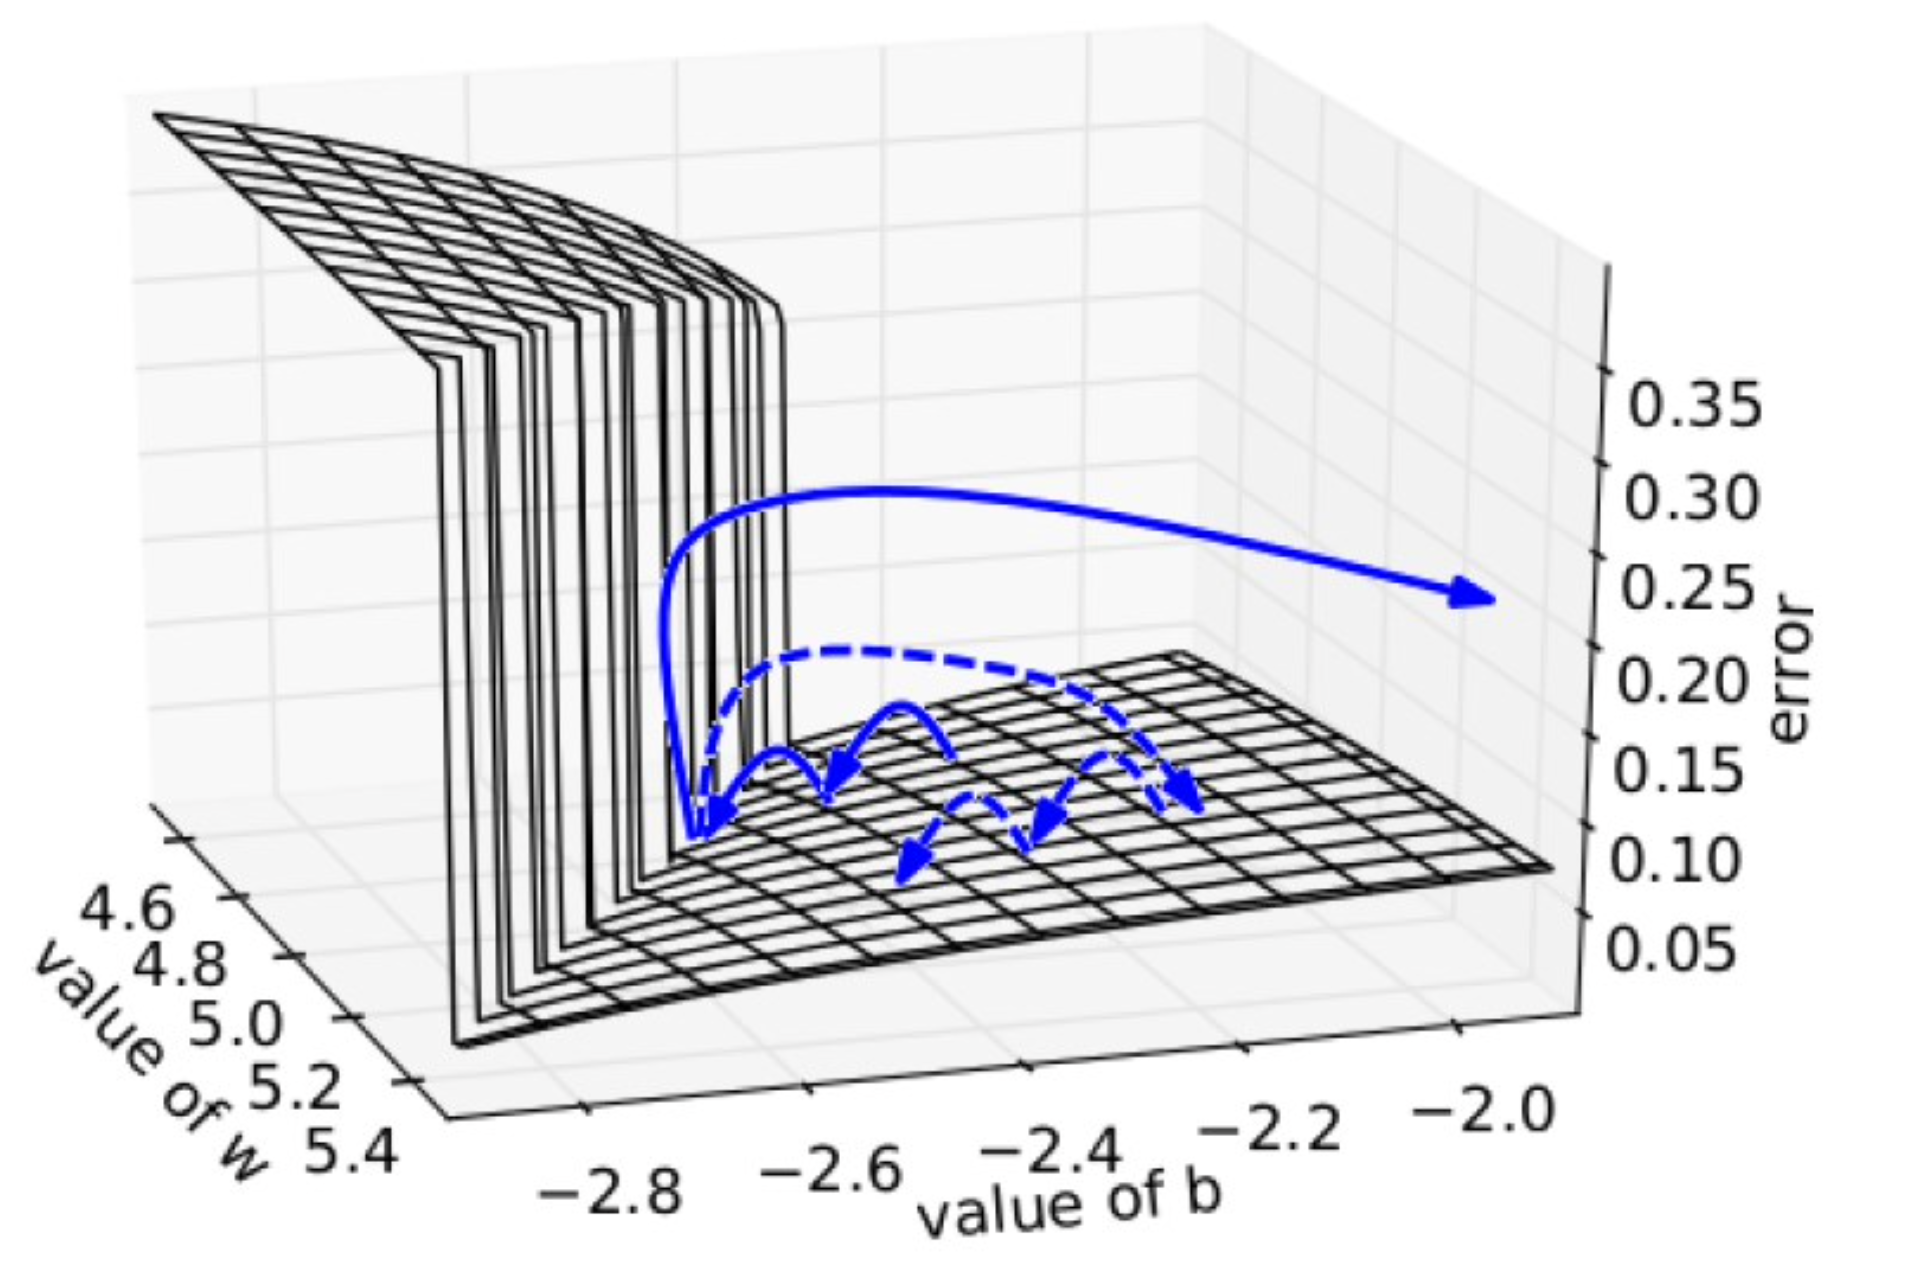
\includegraphics[scale=0.09]{./img/gradient_clipping.png}
		\end{figure}
		\item GRUs and LSTMs
	\end{itemize}
\end{frame}
\begin{frame}{Gated Recurrent Units (GRUs)}
	\begin{itemize}
		\item GRUs are introduced by Cho et al., (2014)
		\item more advanced method for hidden state representation
		\item The key idea behind GRUs is to enable hidden states to capture long distance dependencies
	\end{itemize}
\end{frame}


\begin{frame}{GRUs}
	\centering
	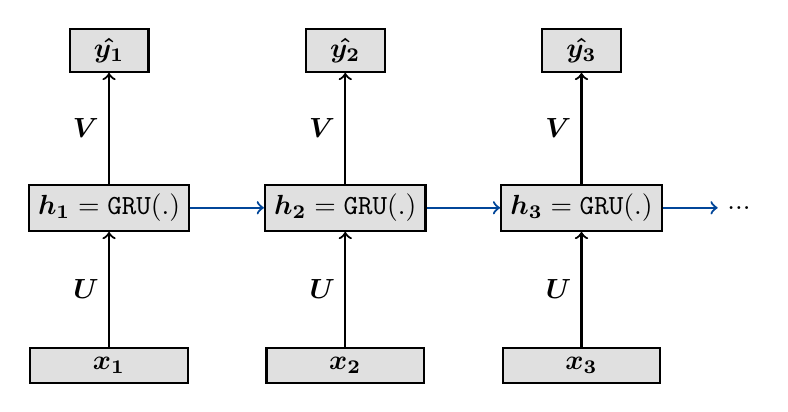
\begin{tikzpicture}
	\tikzset{layer/.style={draw,rectangle, fill=gray!20, thick}}
	\tikzset{edge/.style={->, thick}}
	
	\node(x1) at (0,0) [layer, minimum width=2cm] {$\bm{x_1}$};
	\node(h1) at (0,2) [layer, minimum width=1.5cm] {$\bm{h_1}=\texttt{GRU}(.)$};
	\node(y1_hat) at (0,4) [layer, minimum width=1cm] {$\bm{\hat{y_1}}$};
	\draw[edge](x1) -- node[left]{$\bm{U}$} (h1);
	\draw[edge](h1) -- node[left]{$\bm{V}$} (y1_hat);
	
	
	\node(x2) at (3,0) [layer, minimum width=2cm] {$\bm{x_2}$};
	\node(h2) at (3,2) [layer, minimum width=1.5cm] {$\bm{h_2}=\texttt{GRU}(.)$};
	\node(y2_hat) at (3,4) [layer, minimum width=1cm] {$\bm{\hat{y_2}}$};
	\draw[edge](x2) -- node[left]{$\bm{U}$} (h2);
	\draw[edge](h2) -- node[left]{$\bm{V}$} (y2_hat);
	
	\node(x3) at (6,0) [layer, minimum width=2cm] {$\bm{x_3}$};
	\node(h3) at (6,2) [layer, minimum width=1.5cm] {$\bm{h_3}=\texttt{GRU}(.)$};
	\node(y3_hat) at (6,4) [layer, minimum width=1cm] {$\bm{\hat{y_3}}$};
	\draw[edge](x3) -- node[left]{$\bm{U}$} (h3);
	\draw[edge](h3) -- node[left]{$\bm{V}$} (y3_hat);
	
	\node(etc) at (8,2) [] {...};
	
	\draw[edge, myblue] (h1) --  (h2);
	\draw[edge,myblue] (h2) --  (h3);
	\draw[edge,myblue] (h3) -- (etc);
	
	\end{tikzpicture}
\end{frame}
\begin{frame}
	\centering
	\begin{figure}
		\centering
		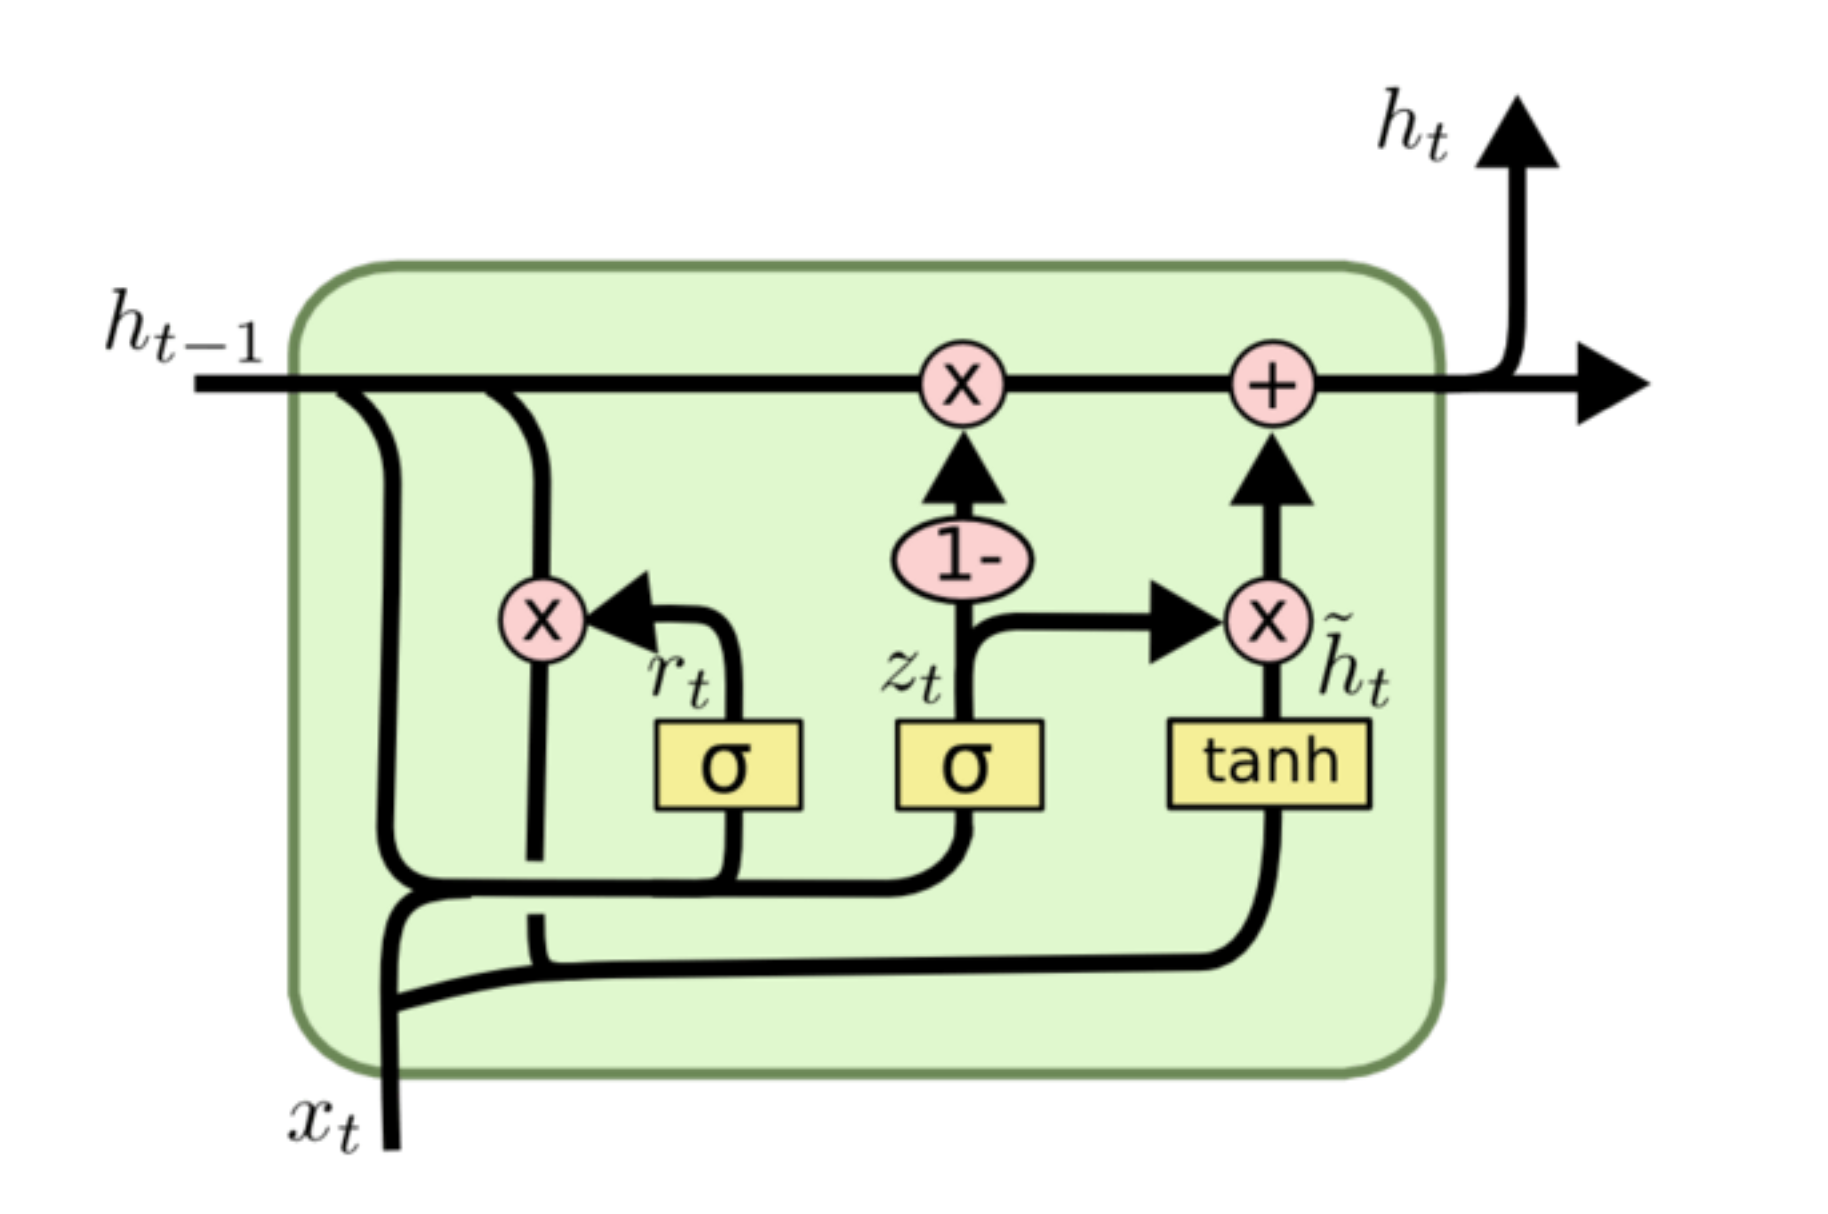
\includegraphics[scale=0.2]{./img/gru.png}
	\end{figure}
	\begin{itemize}
		\item reset gate $r_t = \sigma ( \bm{x_t} \bm{U^{(r)}} + \bm{h_{t-1}} \bm{W^{(r)}} )$
		\item new memory content could be $\bm{\tilde{h}_t} = \texttt{tanh} ( \bm{x_t} \bm{U} + \bm{h_{t-1}} \bm{W} 
		\odot r_t)$ 
		\item update gate $z_t = \sigma ( \bm{x_t} \bm{U^{(z)}} + \bm{h_{t-1}} \bm{W^{(z)}} )$
		\item final memory encodes a combination of current content and its content in the previous time step
		$\bm{h_t} = (1-z_t) \odot \bm{h_{t-1}} + z_t \odot \bm{\tilde{h}_t}$
	\end{itemize}
\end{frame}
\begin{frame}{GRU: Extreme Cases}
	\centering
	\begin{itemize}
		\item reset gate $r_t \in {0,1}$
		\item update gate $z_t \in {0,1}$
		\item If $z_t = 0$
		\begin{itemize}
			\item $\bm{h_t} = (1-z_t) \odot \bm{h_{t-1}} + z_t \odot \bm{\tilde{h}_t}$ 
			\item $\bm{h_t} = \bm{h_{t-1}}$
			\item zero gradients over different time steps 
			\item no vanishing gradients
		\end{itemize}
		\item If $z_t =1$
		\begin{itemize}
			\item $\bm{h_t} = (1-z_t) \odot \bm{h_{t-1}} + z_t \odot \bm{\tilde{h}_t}$ 
			\item $\bm{h_t} = \bm{\tilde{h}_t}$
			\item  $\bm{\tilde{h}_t} = \texttt{tanh} ( \bm{x_t} \bm{U} + \bm{h_{t-1}} \bm{W} \odot r_t)$ 
			\item If $r_t=0$
			\begin{itemize}
				\item $\bm{h_t} = \texttt{tanh}(\bm{x_tU})$ 
				\item forget past
			\end{itemize}
			\item If $r_t =1$
			\begin{itemize}
				\item $\bm{h_t} = \texttt{tanh} ( \bm{x_t} \bm{U} + \bm{h_{t-1}} \bm{W}) $
				\item a standard RNN gate
			\end{itemize}
		\end{itemize}
	\end{itemize}
\end{frame}

\begin{frame}{Long Short-Term Memory (LSTMs)}
	\begin{itemize}
		\item LSTMs were introduced by Hochreiter and Schmidhuber (1997)
		\item LSTMs contains more parameters than what GRU has
	\end{itemize}
\end{frame}

\begin{frame}{LSTM Unit}
	\centering
	\begin{figure}
		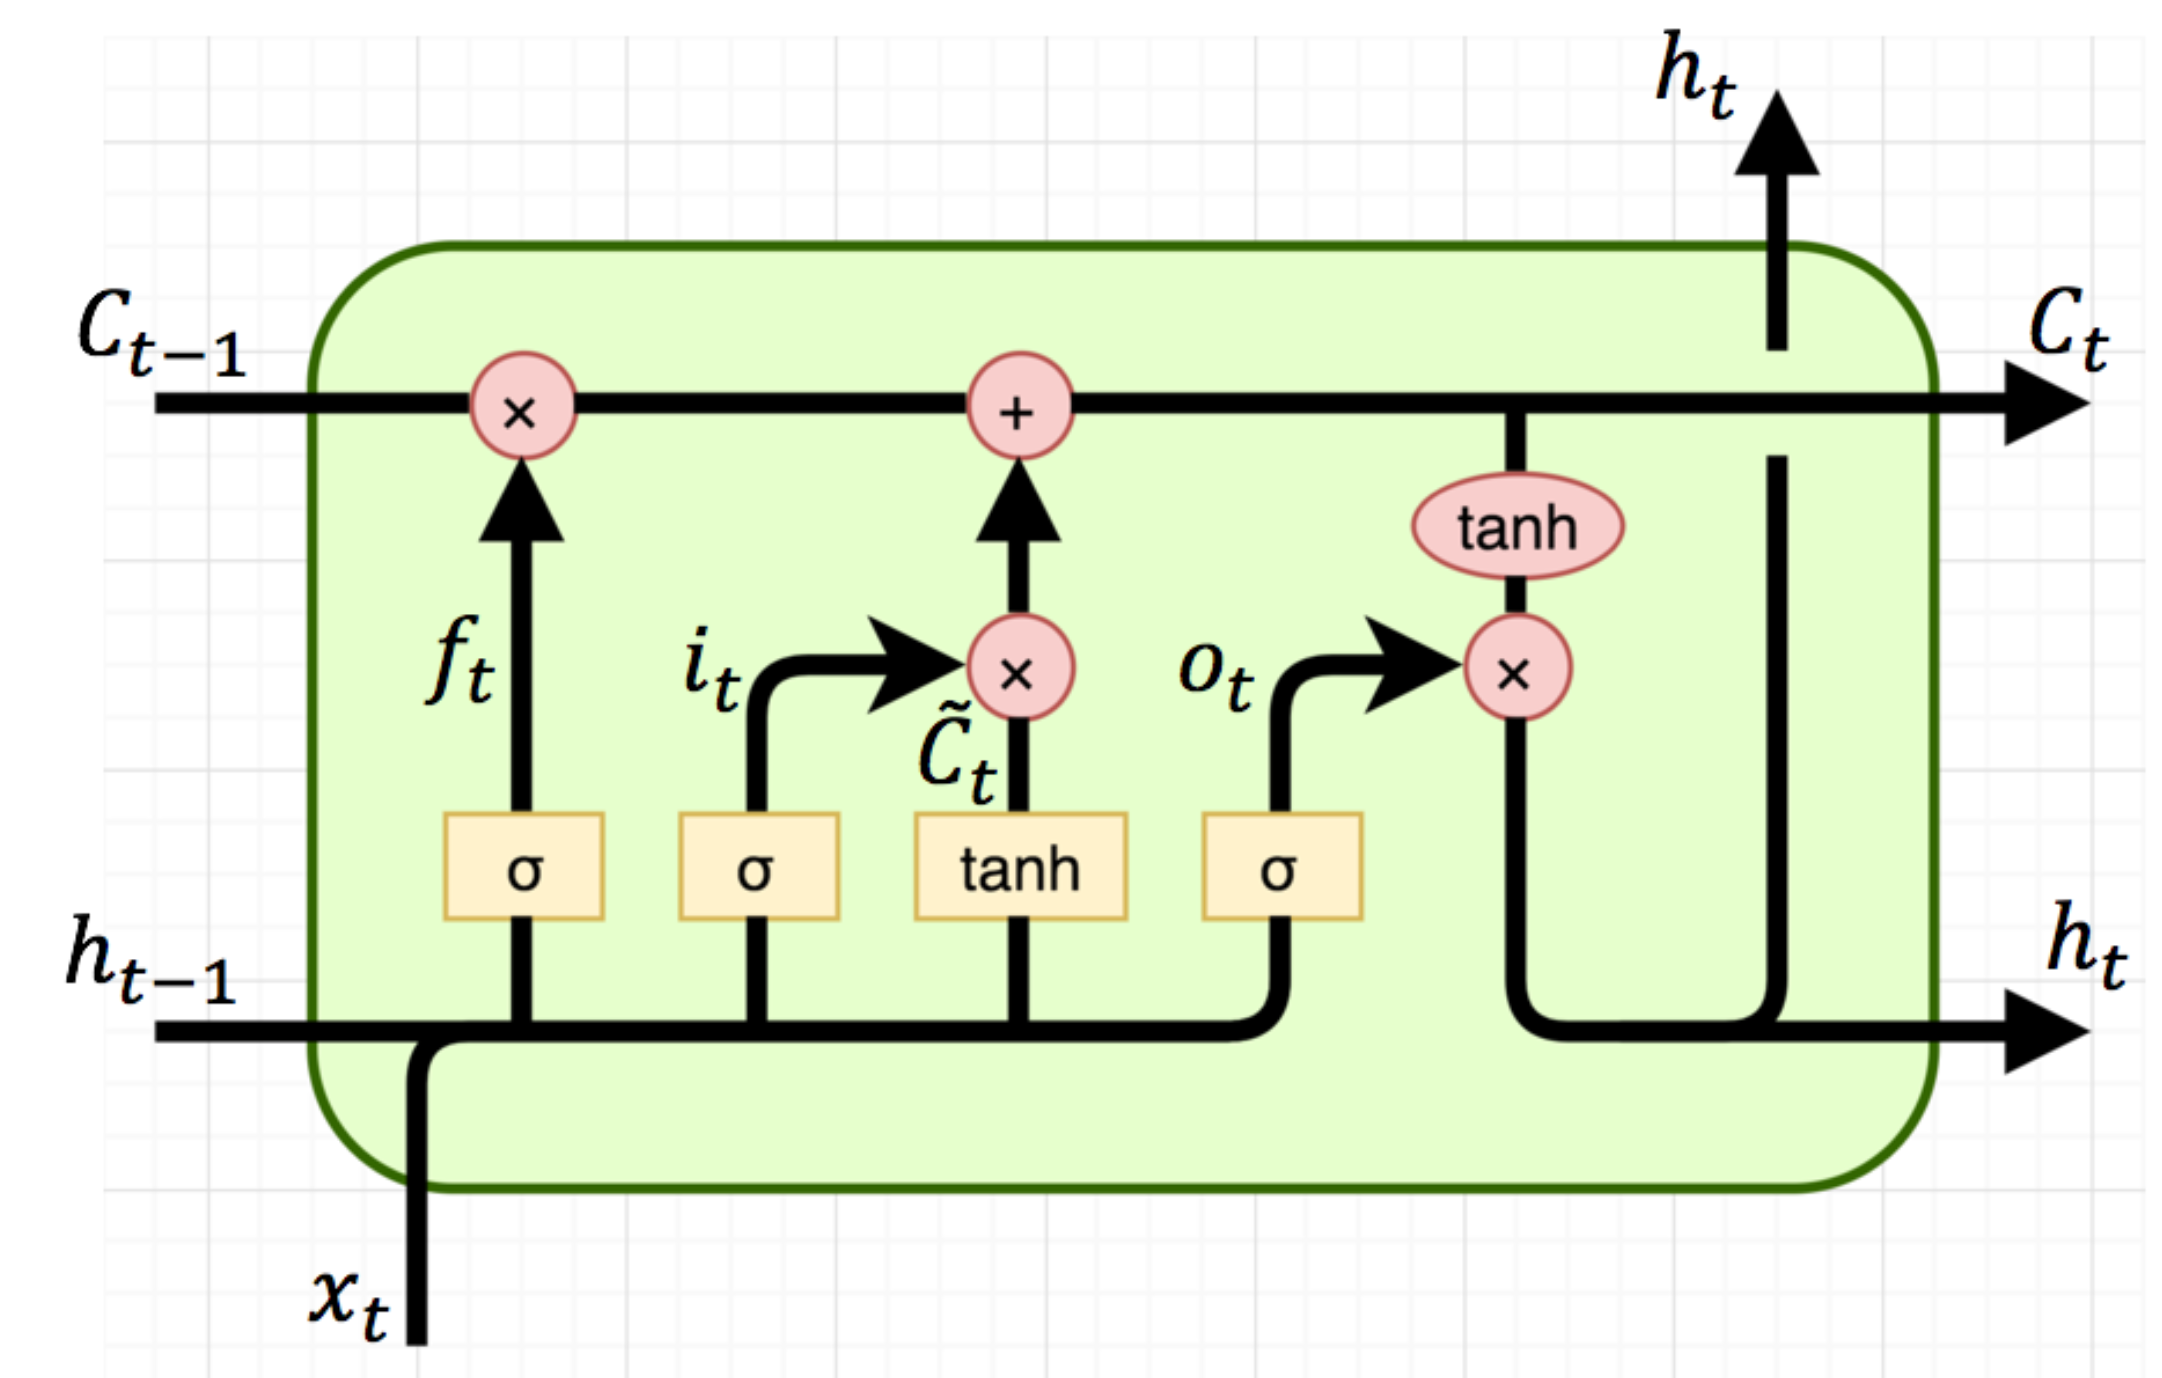
\includegraphics[scale=0.15]{./img/lstm.png}
	\end{figure}
	\begin{itemize}
		\item Input gate (=write gate) $i_t = \sigma \big( \bm{x_tU^{(i)}} + \bm{h_{t-1}W^{(i)}}   \big) $
		\item Forget gate (=reset gate) $f_t = \sigma \big( \bm{x_tU^{(f)}} + \bm{h_{t-1}W^{(f)}}   \big) $
		\item Output gate (=read gate) $o_t = \sigma \big( \bm{x_tU^{(o)}} + \bm{h_{t-1}W^{(o)}}   \big) $
		
		\item New memory cell is $\bm{\tilde{c}_t} = \texttt{tanh} ( \bm{x_tU}+\bm{h_{t-1}W} ) $
		\item Final memory cell is $\bm{c_t} = f_t \odot \bm{c_{t-1}} + i_t \odot \bm{\tilde{c}_t}$
		\item Final hidden state is $\bm{h_t} = o_t \odot \texttt{tanh}(c_t)$
	\end{itemize}
\end{frame}



\begin{frame}{Bidirectional RNNs (BiRNNs)}
	\begin{itemize}
		\item We use two RNNs with two different sets of parameters
		\begin{itemize}
			\item one RNN for processing input symbols from left-to-right
			\item one RNN for processing input symbols from right-to-left
		\end{itemize}
		\item Final representations of each step is the concatenation of the outputs of these RNNs. 
		\begin{itemize}
			\item $\bm{h_t} = [ \bm{\overrightarrow{h_t}}; \bm{\overleftarrow{h_t}}]$
		\end{itemize}
		
		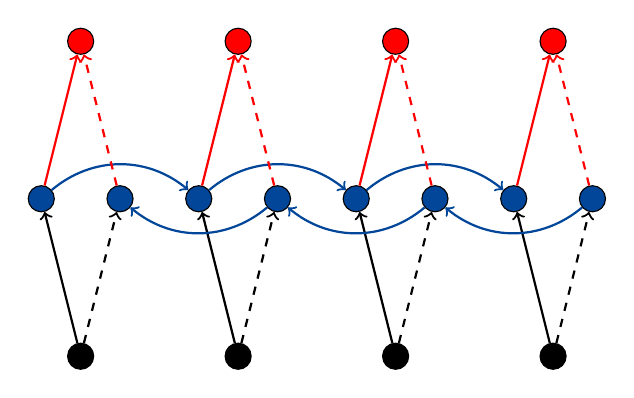
\begin{tikzpicture}
		\tikzset{layer/.style={draw,circle}}
		\tikzset{edge/.style={->, thick}}
		
		\node(x1) at (1,0) [layer,fill=black] {};
		\node(x2) at (3,0) [layer,fill=black] {};
		\node(x3) at (5,0) [layer,fill=black] {};
		\node(x4) at (7,0) [layer,fill=black] {};
		
		\node(h_lr1) at (0.5,2) [layer,fill=myblue] {};
		\node(h_lr2) at (2.5,2) [layer,fill=myblue] {};
		\node(h_lr3) at (4.5,2) [layer,fill=myblue] {};
		\node(h_lr4) at (6.5,2) [layer,fill=myblue] {};
		
		
		\node(h_rl1) at (1.5,2) [layer,fill=myblue] {};
		\node(h_rl2) at (3.5,2) [layer,fill=myblue] {};
		\node(h_rl3) at (5.5,2) [layer,fill=myblue] {};
		\node(h_rl4) at (7.5,2) [layer,fill=myblue] {};
		
		
		\node(y_hat1) at (1,4) [layer,fill=red] {};
		\node(y_hat2) at (3,4) [layer,fill=red] {};
		\node(y_hat3) at (5,4) [layer,fill=red] {};
		\node(y_hat4) at (7,4) [layer,fill=red] {};
		
		\draw[edge] (x1) -- (h_lr1);
		\draw[edge] (x2) -- (h_lr2);
		\draw[edge] (x3) -- (h_lr3);
		\draw[edge] (x4) -- (h_lr4);
		
		\draw[edge, dashed] (x1) -- (h_rl1);
		\draw[edge, dashed] (x2) -- (h_rl2);
		\draw[edge, dashed] (x3) -- (h_rl3);
		\draw[edge, dashed] (x4) -- (h_rl4);
		
		\draw[edge,bend left=40, myblue] (h_lr1) edge (h_lr2);
		\draw[edge,bend left=40, myblue] (h_lr2) edge (h_lr3);            
		\draw[edge,bend left=40, myblue] (h_lr3) edge (h_lr4);
		
		
		\draw[edge,bend left=40, myblue] (h_rl2) edge (h_rl1);
		\draw[edge,bend left=40, myblue] (h_rl3) edge (h_rl2);            
		\draw[edge,bend left=40, myblue] (h_rl4) edge (h_rl3); 
		
		\draw[edge,red] (h_lr1) edge (y_hat1);
		\draw[edge,red] (h_lr2) edge (y_hat2);
		\draw[edge,red] (h_lr3) edge (y_hat3);
		\draw[edge,red] (h_lr4) edge (y_hat4);
		
		
		\draw[edge,red, dashed] (h_rl1) edge (y_hat1);
		\draw[edge,red, dashed] (h_rl2) edge (y_hat2);
		\draw[edge,red, dashed] (h_rl3) edge (y_hat3);
		\draw[edge,red, dashed] (h_rl4) edge (y_hat4);
		\end{tikzpicture} 
	\end{itemize}
\end{frame}

\begin{frame}{Deep BiRNNs}
	\centering
	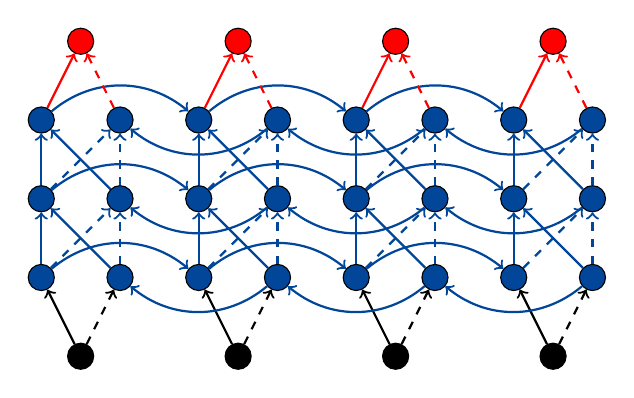
\begin{tikzpicture}
	\tikzset{layer/.style={draw,circle}}
	\tikzset{edge/.style={->, thick}}
	
	\node(x1) at (1,0) [layer,fill=black] {};
	\node(x2) at (3,0) [layer,fill=black] {};
	\node(x3) at (5,0) [layer,fill=black] {};
	\node(x4) at (7,0) [layer,fill=black] {};
	
	\node(h_lr1) at (0.5,1) [layer,fill=myblue] {};
	\node(h_lr2) at (2.5,1) [layer,fill=myblue] {};
	\node(h_lr3) at (4.5,1) [layer,fill=myblue] {};
	\node(h_lr4) at (6.5,1) [layer,fill=myblue] {};
	
	
	\node(h_rl1) at (1.5,1) [layer,fill=myblue] {};
	\node(h_rl2) at (3.5,1) [layer,fill=myblue] {};
	\node(h_rl3) at (5.5,1) [layer,fill=myblue] {};
	\node(h_rl4) at (7.5,1) [layer,fill=myblue] {};
	
	
	\draw[edge] (x1) -- (h_lr1);
	\draw[edge] (x2) -- (h_lr2);
	\draw[edge] (x3) -- (h_lr3);
	\draw[edge] (x4) -- (h_lr4);
	
	\draw[edge, dashed] (x1) -- (h_rl1);
	\draw[edge, dashed] (x2) -- (h_rl2);
	\draw[edge, dashed] (x3) -- (h_rl3);
	\draw[edge, dashed] (x4) -- (h_rl4);
	
	\draw[edge,bend left=40, myblue] (h_lr1) edge (h_lr2);
	\draw[edge,bend left=40, myblue] (h_lr2) edge (h_lr3);            
	\draw[edge,bend left=40, myblue] (h_lr3) edge (h_lr4);
	\draw[edge,bend left=40, myblue] (h_rl2) edge (h_rl1);
	\draw[edge,bend left=40, myblue] (h_rl3) edge (h_rl2); 
	\draw[edge,bend left=40, myblue] (h_rl4) edge (h_rl3); 
	
	
	\node(h2_lr1) at (0.5,2) [layer,fill=myblue] {};
	\node(h2_lr2) at (2.5,2) [layer,fill=myblue] {};
	\node(h2_lr3) at (4.5,2) [layer,fill=myblue] {};
	\node(h2_lr4) at (6.5,2) [layer,fill=myblue] {};
	
	
	\node(h2_rl1) at (1.5,2) [layer,fill=myblue] {};
	\node(h2_rl2) at (3.5,2) [layer,fill=myblue] {};
	\node(h2_rl3) at (5.5,2) [layer,fill=myblue] {};
	\node(h2_rl4) at (7.5,2) [layer,fill=myblue] {};
	
	\draw[edge, myblue] (h_lr1) edge (h2_lr1);
	\draw[edge, myblue] (h_rl1) edge (h2_lr1);
	\draw[edge, myblue] (h_lr2) edge (h2_lr2);
	\draw[edge, myblue] (h_rl2) edge (h2_lr2);
	\draw[edge, myblue] (h_lr3) edge (h2_lr3);
	\draw[edge, myblue] (h_rl3) edge (h2_lr3);
	\draw[edge, myblue] (h_lr4) edge (h2_lr4);
	\draw[edge, myblue] (h_rl4) edge (h2_lr4);
	
	
	\draw[edge, myblue, dashed] (h_lr1) edge (h2_rl1);
	\draw[edge, myblue, dashed] (h_rl1) edge (h2_rl1);
	\draw[edge, myblue, dashed] (h_lr2) edge (h2_rl2);
	\draw[edge, myblue, dashed] (h_rl2) edge (h2_rl2);
	\draw[edge, myblue, dashed] (h_lr3) edge (h2_rl3);
	\draw[edge, myblue, dashed] (h_rl3) edge (h2_rl3);
	\draw[edge, myblue, dashed] (h_lr4) edge (h2_rl4);
	\draw[edge, myblue, dashed] (h_rl4) edge (h2_rl4);
	
	\draw[edge,bend left=40, myblue] (h2_lr1) edge (h2_lr2);
	\draw[edge,bend left=40, myblue] (h2_lr2) edge (h2_lr3);            
	\draw[edge,bend left=40, myblue] (h2_lr3) edge (h2_lr4);
	\draw[edge,bend left=40, myblue] (h2_rl2) edge (h2_rl1);
	\draw[edge,bend left=40, myblue] (h2_rl3) edge (h2_rl2); 
	\draw[edge,bend left=40, myblue] (h2_rl4) edge (h2_rl3); 
	
	
	\node(h3_lr1) at (0.5,3) [layer,fill=myblue] {};
	\node(h3_lr2) at (2.5,3) [layer,fill=myblue] {};
	\node(h3_lr3) at (4.5,3) [layer,fill=myblue] {};
	\node(h3_lr4) at (6.5,3) [layer,fill=myblue] {};
	
	
	\node(h3_rl1) at (1.5,3) [layer,fill=myblue] {};
	\node(h3_rl2) at (3.5,3) [layer,fill=myblue] {};
	\node(h3_rl3) at (5.5,3) [layer,fill=myblue] {};
	\node(h3_rl4) at (7.5,3) [layer,fill=myblue] {};
	
	\draw[edge, myblue] (h2_lr1) edge (h3_lr1);
	\draw[edge, myblue] (h2_rl1) edge (h3_lr1);
	\draw[edge, myblue] (h2_lr2) edge (h3_lr2);
	\draw[edge, myblue] (h2_rl2) edge (h3_lr2);
	\draw[edge, myblue] (h2_lr3) edge (h3_lr3);
	\draw[edge, myblue] (h2_rl3) edge (h3_lr3);
	\draw[edge, myblue] (h2_lr4) edge (h3_lr4);
	\draw[edge, myblue] (h2_rl4) edge (h3_lr4);
	
	
	\draw[edge, myblue, dashed] (h2_lr1) edge (h3_rl1);
	\draw[edge, myblue, dashed] (h2_rl1) edge (h3_rl1);
	\draw[edge, myblue, dashed] (h2_lr2) edge (h3_rl2);
	\draw[edge, myblue, dashed] (h2_rl2) edge (h3_rl2);
	\draw[edge, myblue, dashed] (h2_lr3) edge (h3_rl3);
	\draw[edge, myblue, dashed] (h2_rl3) edge (h3_rl3);
	\draw[edge, myblue, dashed] (h2_lr4) edge (h3_rl4);
	\draw[edge, myblue, dashed] (h2_rl4) edge (h3_rl4);
	
	\draw[edge,bend left=40, myblue] (h3_lr1) edge (h3_lr2);
	\draw[edge,bend left=40, myblue] (h3_lr2) edge (h3_lr3);            
	\draw[edge,bend left=40, myblue] (h3_lr3) edge (h3_lr4);
	\draw[edge,bend left=40, myblue] (h3_rl2) edge (h3_rl1);
	\draw[edge,bend left=40, myblue] (h3_rl3) edge (h3_rl2); 
	\draw[edge,bend left=40, myblue] (h3_rl4) edge (h3_rl3); 
	
	
	
	\node(y_hat1) at (1,4) [layer,fill=red] {};
	\node(y_hat2) at (3,4) [layer,fill=red] {};
	\node(y_hat3) at (5,4) [layer,fill=red] {};
	\node(y_hat4) at (7,4) [layer,fill=red] {};
	
	
	\draw[edge,red] (h3_lr1) edge (y_hat1);
	\draw[edge,red] (h3_lr2) edge (y_hat2);
	\draw[edge,red] (h3_lr3) edge (y_hat3);
	\draw[edge,red] (h3_lr4) edge (y_hat4);
	
	
	\draw[edge,red, dashed] (h3_rl1) edge (y_hat1);
	\draw[edge,red, dashed] (h3_rl2) edge (y_hat2);
	\draw[edge,red, dashed] (h3_rl3) edge (y_hat3);
	\draw[edge,red, dashed] (h3_rl4) edge (y_hat4);
	
	\end{tikzpicture} 
\end{frame}

\begin{frame}{RNNs With  Output Connections}
	\centering
	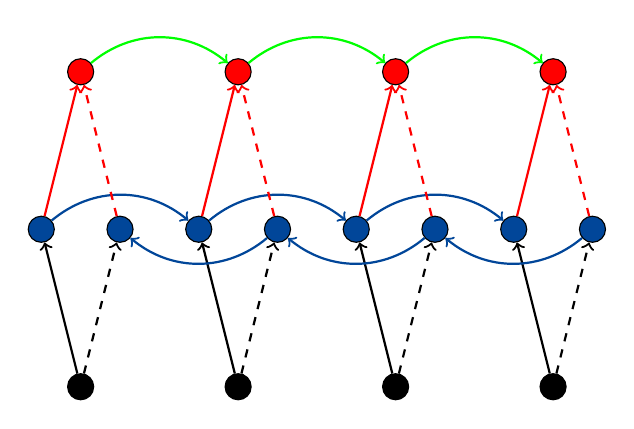
\begin{tikzpicture}
	\tikzset{layer/.style={draw,circle}}
	\tikzset{edge/.style={->, thick}}
	
	\node(x1) at (1,0) [layer,fill=black] {};
	\node(x2) at (3,0) [layer,fill=black] {};
	\node(x3) at (5,0) [layer,fill=black] {};
	\node(x4) at (7,0) [layer,fill=black] {};
	
	\node(h_lr1) at (0.5,2) [layer,fill=myblue] {};
	\node(h_lr2) at (2.5,2) [layer,fill=myblue] {};
	\node(h_lr3) at (4.5,2) [layer,fill=myblue] {};
	\node(h_lr4) at (6.5,2) [layer,fill=myblue] {};
	
	
	\node(h_rl1) at (1.5,2) [layer,fill=myblue] {};
	\node(h_rl2) at (3.5,2) [layer,fill=myblue] {};
	\node(h_rl3) at (5.5,2) [layer,fill=myblue] {};
	\node(h_rl4) at (7.5,2) [layer,fill=myblue] {};
	
	
	\node(y_hat1) at (1,4) [layer,fill=red] {};
	\node(y_hat2) at (3,4) [layer,fill=red] {};
	\node(y_hat3) at (5,4) [layer,fill=red] {};
	\node(y_hat4) at (7,4) [layer,fill=red] {};
	
	\draw[edge] (x1) -- (h_lr1);
	\draw[edge] (x2) -- (h_lr2);
	\draw[edge] (x3) -- (h_lr3);
	\draw[edge] (x4) -- (h_lr4);
	
	\draw[edge, dashed] (x1) -- (h_rl1);
	\draw[edge, dashed] (x2) -- (h_rl2);
	\draw[edge, dashed] (x3) -- (h_rl3);
	\draw[edge, dashed] (x4) -- (h_rl4);
	
	\draw[edge,bend left=40, myblue] (h_lr1) edge (h_lr2);
	\draw[edge,bend left=40, myblue] (h_lr2) edge (h_lr3);            
	\draw[edge,bend left=40, myblue] (h_lr3) edge (h_lr4);
	
	
	\draw[edge,bend left=40, myblue] (h_rl2) edge (h_rl1);
	\draw[edge,bend left=40, myblue] (h_rl3) edge (h_rl2);            
	\draw[edge,bend left=40, myblue] (h_rl4) edge (h_rl3); 
	
	\draw[edge,red] (h_lr1) edge (y_hat1);
	\draw[edge,red] (h_lr2) edge (y_hat2);
	\draw[edge,red] (h_lr3) edge (y_hat3);
	\draw[edge,red] (h_lr4) edge (y_hat4);
	
	
	\draw[edge,red, dashed] (h_rl1) edge (y_hat1);
	\draw[edge,red, dashed] (h_rl2) edge (y_hat2);
	\draw[edge,red, dashed] (h_rl3) edge (y_hat3);
	\draw[edge,red, dashed] (h_rl4) edge (y_hat4);
	
	\draw[edge,green, bend left=40] (y_hat1) edge (y_hat2);
	\draw[edge,green, bend left=40] (y_hat2) edge (y_hat3);
	\draw[edge,green, bend left=40] (y_hat3) edge (y_hat4);
	
	
	\end{tikzpicture} 
\end{frame}


\begin{frame}{Applications of RNNs in NLP}
	\begin{itemize}
		\item Part-of-Speech (POS) tagging
		\begin{itemize}
			\item input: a sequence of words 
			\item output: a sequence of POS tags (NOUN, VERB, ...)
		\end{itemize}
		\item Named Entity Recognition (NER)
		\begin{itemize}
			\item input: a sequence of words 
			\item output: a sequence of NER tags (B-PER, I-PER, O, B-LOC, I-LOC,...)
		\end{itemize}
		\item Language Modeling (LM)
		\begin{itemize}
			\item input: a sequence of words 
			\item output: a sequence of words $y_t = x_{t-1}$
		\end{itemize}
		
		\item Sentence Classification
		\begin{itemize}
			\item input: a sequence of words 
			\item output: one label for the whole sequence
			\item trick: use the hidden state of the last step to represent the whole sentence  
		\end{itemize}
	\end{itemize}
\end{frame}


%%%%%%%%%%%%%%%%%%%%%%%%%%%%%%%%%%
\begin{frame}{Summary}
	\begin{itemize}
		\item RNNs are used mostly for sequence prediction.
		\item RNNs face with vanishing and exploding gradient issues. 
		\item Vanishing and Exploding Gradients in RNNs
		\item LSTMs and GRUs
		\item Applications of RNNs
	\end{itemize}
\end{frame}



\begin{frame}{License and credits}

\begin{columns}
	\begin{column}{0.7\textwidth}
		Licensed under Creative Commons Attribution-ShareAlike 4.0 International (CC BY-SA 4.0)
	\end{column}
	\begin{column}{0.2\textwidth}
		
\includegraphics[width=0.9\linewidth]{img/cc-by-sa-icon.pdf}
	\end{column}
\end{columns}

\bigskip

Credits

\begin{scriptsize}
	
Ivan Habernal, Mohsen Mesgar, Steffen Eger

Content from the ACL Anthology licensed under CC-BY \url{https://www.aclweb.org/anthology}

\end{scriptsize}

\end{frame}

\begin{frame}[allowframebreaks]{References}
\printbibliography
%  \bibliography{bibliography}
%  \bibliographystyle{abbrv}
\end{frame}

\end{document}

